\section{Vibration sensor}
\begin{figure}[H]
    \centering
    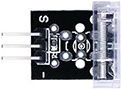
\includegraphics[angle=0, keepaspectratio=true, scale=1, width=200px, height=200px]{images/vibration.jpg}
    \caption{Caption}
\end{figure}
\subsection*{Description}
This module operates on the same principle as the shock sensor and has a very small sensitive spring which absorbs vibrations.
\subsection*{Pin mapping}
This pin mapping corresponds to the pins from left to right with the module pins facing towards you.
\begin{table}[H]
    \centering
    \begin{tabular}{|c|c|c|c|c|}
    \hline
    Index &Label &Type &Name &Description\\ \hline
    0 &S &Digital output &D0 &\\ \hline
    1 & &Source voltage &$V+$ &Module source voltage ($5V$)\\ \hline
    2 &- &Ground &GND &\\ \hline
    \end{tabular}
    %\caption{Caption}
    %\label{tab:my_label}
\end{table}
\subsection*{Operation}
When the module is stable the voltage of the digital output pin D0 is low. When the module experiences signification vibration the voltage of D0 will be set to high.
\subsection*{Code}
Refer to listing \ref{python_vibration}.
%\lstinputlisting[caption=test]{laser.py}